\documentclass[preprint2,hidelinks]{emulateapj}

\usepackage{url}
\usepackage{multirow}
\usepackage{amsmath}
\usepackage{xcolor}
\usepackage{hyperref}
\usepackage{affils}
%\citestyle{aa}

%\bibliographystyle{apj_w_etal}

\newcommand{\etal}{{et al.\/}}
\newcommand{\Prob}{\mathtt{P}}
\newcommand{\logL}{\log\mathcal{L}}
\newcommand{\unit}[1]{\footnotesize #1}
\newcommand{\PAPER}{\mathrm{PAPER}}
\newcommand{\hMpci}{h\ {\rm Mpc}^{-1}}

%%define graphics path to search for images
\graphicspath{{./data/}}

\newcommand{\Nconf}{31}
\newcommand{\Nsrc}{32}
\definecolor{orange}{RGB}{255,127,0}
\tabletypesize{\scriptsize}

	% End definitions

%\slugcomment{DRAFT: \today}

\shorttitle{PAPER-64 III: Information loss in OQEs}
\shortauthors{Kolopanis et al.}

\begin{document}


\title{PAPER-64 III: Information Loss In Optimal Quadratic Estimation of the 21cm Power Spectrum}

\DeclareAffil{1}{Astronomy Dept., U. California, Berkeley CA}
\DeclareAffil{2}{Radio Astronomy Lab., U. California, Berkeley CA}
\DeclareAffil{3}{Dept. of Physics, Massachusetts Inst. of Tech., Cambridge MA}
\DeclareAffil{4}{Physics Dept.  U. Washington, Seattle WA}
\DeclareAffil{5}{Berkeley Center for Cosmological Physics, Berkeley, CA} 
\DeclareAffil{6}{Dept. of Physics and Astronomy, U. Penn., Philadelphia PA} 
\DeclareAffil{7}{Dept. of Electrical and Computer Engineering, U. Virginia, Charlottesville VA}
\DeclareAffil{8}{National Radio Astronomy Obs., Charlottesville VA}
\DeclareAffil{9}{Dept. of Astronomy, U. Virginia, Charlottesville VA}
\DeclareAffil{10}{Square Kilometer Array, S. Africa, Cape Town South Africa}
\DeclareAffil{11}{Dept. of Physics and Electronics, Rhodes University}
\DeclareAffil{12}{Harvard-Smithsonian Cen. for Astrophysics, Cambridge MA}
\DeclareAffil{13}{National Radio Astronomy Obs., Socorro NM}
\DeclareAffil{14}{Cavendish Lab., Cambridge UK}
\DeclareAffil{15}{School of Earth and Space Exploration, Arizona State U., Tempe AZ}
\DeclareAffil{16}{Department of Physics, Arizona State U., Tempe AZ}




\affilauthorlist{
Matthew J. Kolopanis\affils{15,16},
Daniel C. Jacobs\affils{15},
Carina Cheng\affils{1},
Aaron R. Parsons\affils{1,2},
Zaki S. Ali\affils{1}, 
Haoxuan Zheng\affils{3},
Jonathan C. Pober\affils{4}, 
Adrian Liu\affils{1,5},
James E. Aguirre\affils{6},
Richard F. Bradley\affils{7,8,9},
Gianni Bernardi\affils{10,11,12}, 
Chris L. Carilli\affils{13,14},
David R. DeBoer\affils{2}, 
Matthew R. Dexter\affils{2},
Jasper Grobbelaar\affils{10},
Jasper Horrell\affils{10},
Judd Bowman\affils{15}, 
Pat Klima\affils{8},
David H. E. MacMahon\affils{2},
Matthys Maree\affils{10},
David F. Moore\affils{6},
Nima Razavi\affils{14},
Irina I. Stefan\affils{14},
William P. Walbrugh\affils{10},
Andre Walker\affils{10}
}
%\tableofcontents

\begin{abstract}
The use of Optimal Quadratic Estimators in power spectrum estimation is a popular choice among recent radio arrays. Properly modeling and accounting for covariance among measurement channels allows for lossless power spectrum estimation with this technique; however the use of empirically estimated covariance matrices has been shown to cause over fitting of noise-like terms and as a result information loss. We show previous investigations have not properly identified and characterized this effect and offer a new method to account for and overcome information loss in power spectrum estimation. The application of this method to PAPER data is presented in our accompanying paper Kolopanis et al (in prep).

%We present new limits on the power spectrum of 21cm emission from the 64-element Donald C. Baker Precision Array for Probing the Epoch of Reionization ($\PAPER$). This work extends the previous upper limits by \citet{ali_et_al2015}. We find improvements by a factor of as much as 4 in sensitivity compared to previous works near redshifts $z=10.87$, $9.92$, $8.91$, $8.12$, and $7.48$. These limits continue to support evidence against extremely cold re-heating scenarios discussed in \citet{pober_et_al2015} and provide the lowest limit to constrain pre-reionization heating and early reionization scenarios assuming fiducal models \citep{robertson_et_al2013,robertson_et_al2015}. We will continue to discuss the impacts on our understanding of the Epoch of Reionization in Jacobs et al 2016 (in prep).
\end{abstract}
\maketitle

\section{Introduction}\label{sec:intro}{
\setcounter{footnote}{0}
The anticipated detection of the 21cm power spectrum will provide 
new information about the evolution of cosmic hydrogen through the 
dark ages and the first types of luminous bodies in our universe. Many radio experiments are attempting to detect this signal include
the Precision Array for Probing the Epoch of Reionizaiton ($\PAPER$\footnote{\url{eor.berkeley.edu}}; \citealt{parsons_et_al2010}), the Giant Metre-wave Radio Telescope (GMRT; \citealt{paciga_et_al2013}), the Low Frequency Array (LOFAR \footnote{\url{www.lofar.org}}; \citealt{yatawatta_et_al2013} ), the Murchison Widefield Array (MWA\footnote{\url{mwatelescope.org}}; \citealt{bowman_et_al2012}), and the upcoming Hydrogen Epoch of Reionization Array (HERA\footnote{\url{reionization.org}}; \citealt{pober_et_al2014};). 

The theoretical predictions for the foregrounds faced by these telescopes can be found in \citet{morales_wyithe2010} and \citet{pritchard_loeb2012}. A review of the physics of reionization is found in \citet{furlanetto_et_al2006}.


A characteristic region of Fourier space is expected to be 
free of Foreground signals and ideal for EoR analysis. This "EoR 
window" consists of a region where spectrally smooth foregrounds
do not contaminate the otherwise isotropic cosmological 21cm 
signal\citep{bowman_et_al2009,morales_et_al2006a}. 

The EoR Window is accompanied by an area in Fourier space of 
foreground leakage has been identified as a result of 
instrumental mode mixing \citep{parsons_et_al2012b}.
This leakage sends some spectrally smooth foregrounds 
to high Fourier modes resulting in a "wedge" like shape
\citep{pober_et_al2013,nithya_et_al2013,nithya_et_al2015a,
nithya_et_al2015b,trott_et_al2012,liu_et_al2014a,liu_et_al2014b,
hazelton_et_al2013,morales_et_al2012,vedantham_et_al2012,
datta_et_al2010}. 
Foregrounds can extend beyond the horizon level as a result
 of two effects described in \citet{pober_et_al2012}: 
 side lob power and the the extension of sources which are not
 entirely spectrally smooth beyond the physical horizon for a 
 baseline. 
 
 A number of techniques are being investigated to 
remove foreground contamination from both point sources and 
diffuse structure in both image and Fourier domains
\citep{beardsley_et_al2016, pober_et_al2016,trott_et_al2012} and
 Line et al. (in review). 
Aside from removing foreground contaminations, some analysis pipelines attempt to exploit the isolation of the foreground wedge 
and focus their analysis in the "EoR window" 
as a way to avoid foregrounds
 \citep{jacobs_et_al2015,jacobs_et_al2016,trott_et_al2016,
 dillon_et_al2013a,dillon_et_al2015,trott_2014,
 ali_et_al2015,parsons_et_al2014}. 
 
 Many so called "foreground avoidance" techniques rely on the use of 
 an Optimal Quadratic Estimator of the 21cm power spectrum (\citealt{ali_et_al2015} hereafter A15, 
 \citealt{liu_tegmark2011,dillon_et_al2013a,
 dillon_et_al2015,liu_et_al2014a,
 liu_et_al2014b,trott_et_al2012}). These OQEs rely on empirical estimation of data's covariance and as a result may produce signal loss due to over fitting of noise ( A15, \citet{dillon_et_al2015,switzer_liu2014}). Some techniques have been proposed to avoid information loss like the use of eigenmode projection \citep{dillon_et_al2015} or reducing temporal covariance through sub-optimal filtering in A15. 
 
 We find, however, the characterization and presence of information loss in these studies is insufficient and the effect is more prevalent that previously expected. Our investigation focuses on the technique and data used in A15. We offer a new method do characterize and account for these effects in power spectrum estimation using OQEs.


This paper is organized as follows: we provide an review of the mathematics of OQE's in \autoref{sec:oqe}. Our investigation of information loss and new method to overcome this effect is described in \autoref{sec:sigloss}. We conclude with a discussion of these findings in \autoref{sec:discussion}.
}


\begin{figure}[t]
\centering
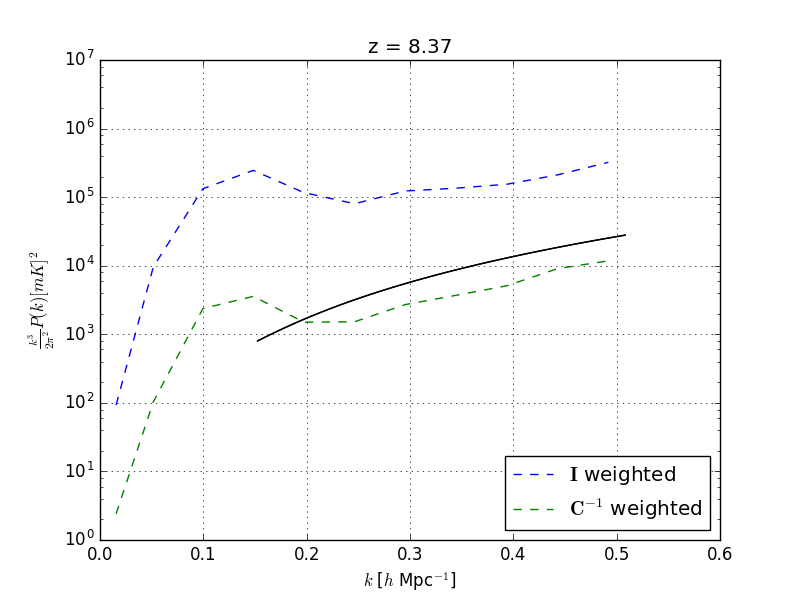
\includegraphics[width=.45\textwidth]{ali_upperlims.png}
\caption{2 sigma upper limits on the 21cm power spectrum using the A15 data. Blue line indicates the power spectrum estimate when no inverse covariance weighting is applied. Green indicates the power spectrum estimate with inverse covariance weighting applied. The expected 2-sigma noise level for each filter's total integration time is given in black. The presence of data below the theoretical lower noise bound may be indicative of information loss \label{fig:ali_pi_vs_pc}}
\end{figure}

\section{The Optimal Quadratic Estimator}\label{sec:oqe}{

}

\section{Information loss in OQEs}\label{sec:sigloss}{
An OQE is traditionally regarded as a lossless power spectrum estimator \citep{tegmark1997}, but A15, \citet{dillon_et_al2015} and \citet{switzer_liu2014} describe how the use of this kind of estimator with empirically estimated covariance matrices can lead to information loss. 

To summarize, lossless estimation requires \emph{a priori} knowledge of the statistics of the covariance matrix $\mathbf{C}$ but estimating $\mathbf{C}$ empirically fundamentally violates this assumption.
As a result, random fluctuations in the data from noise may cause statistically independent sky measurements to appear covariant and thus be down-weighted during power spectrum estimation.


 Our investigation of potential signal loss in our power spectrum estimator begins by running data filtered by the FRF used in A15 and the optimal FRF through the power spectrum pipeline and comparing the relative amplitudes of the estimates with and without the inverse covariance weighting. The $2\sigma$ upper limits from both the inverse covariance weighted data (green) and non-weighted data (blue) from the A15 FRF and the optimal FRF are displayed in \autoref{fig:optimal_vs_ali}. Each panel also contains the $2\sigma$ theoretical noise sensitivity for each FRF computed using the 21cmSense package \citep{pober_et_al2013}. 
 
  Even with perfect foreground removal, a lossless power spectrum estimator would not be able to produce results below the thermal noise level. A possible solution is a miscalculation of the black curves in \autoref{fig:optimal_vs_ali}, however we continue our investigation assuming the thermal noise calculations from \citet{pober_et_al2013} are valid.
  % We also focus our analysis on the use of the optimal FRF since the effect appears to be not heavily dependent on the choice of FRF.
 
 We then perform Monte-Carlo simulations of a Gaussian temperature field with a flat amplitude $P(k)$ over 60 sky realizations for all input signal levels in the range $[10^{4},10^{13}]\ (mK)^{2}$. In A15, the covariance of the data + injected sky signal was only applied to the injected sky signal to determine what loss would occur to this signal if it existed in the data.
 
  We apply the covariance matrix to the sum of data and injected signal to investigate the possibility of total power loss before and after the application of the OQE. For noise limited data being processed with a lossless power spectrum estimator, the total output power of data + injected sky signal should lay along the sum of the expected noise level (green dashed line) and the simulated sky signal in \autoref{fig:sigloss_data}.
  
  The application of this method to the A15 data the the optimally FRF data both is is shown in \autoref{fig:sigloss_data}. This figure illustrate loss for high values of $P_{inj}$ but at lower values of $P_{in}$ it is difficult to discern whether it is indeed suffering from information loss. While the power spectrum estimates in this regime do reside below the non-covariance weighted ($\mathbf{I}$ weighted) power spectra for the data, they are still close to the theoretical noise level. As a result it is difficult to discern between this being a result of information loss or the proper down-weighting of foreground signals.
 %The expected thermal noise level for $\PAPER$-$64$ is represented by the dashed green line.
  To further address this potential issue, the simulation is repeated with simulated visibilities consisting of a white noise signal instead of the observed data. For white noise visibilities, $\mathbf{C}$ should converge to $\mathbf{I}$ multiplied by a scalar quantity (the input noise power). The expected result from applying the Monte-Carlo simulation described above would be identical input and output power for all injected sky signals. The disagreement between these quantities and the similar output shapes of \autoref{fig:sigloss_data} and \autoref{fig:sigloss_noise} indicate the use of empirically estimated covariance matrices in this application of and OQE are causing signal loss. 

	To overcome the effects of signal loss in our power spectrum estimator, we interpret data points and their error bars for each k-bin and injected sky signal as probability distributions. We then compute the probability for each sky signal that the output power of the Monte-Carlo simulations would be observed above the $1\sigma$ upper bounds of the data's power spectrum in each k-bin. This is interpreted as the probability that an underlying 21cm background signal of level $P_{inj}$ would have been detected if present in the data.
	
	A hyperbolic tangent is fit to the probability of detection as a function of $P_{inj}$, from this an arbitrary level of confidence that an underlying signal would be detected can be assigned. We interpret this confidence level as our signal loss corrected upper limits.
 
 %When the input and output power spectra of these simulations are related by a monotonically increasing function over the observed power levels, it is possible to recover a maximum correction factor for each redshift bin.  This effect and the process of recovering correction factors is discussed in detail in A15.
 
% As shown in Figure \ref{fig:sigloss},  The respective correction factors for associated signal loss in the z$= 10.87,\ 9.92,\ 8.91,\ 8.12, \text{ and } 7.48$ redshift bins we recover are $1.62,\ 1.35,\ 1.30,\ 1.28, \text{ and } 1.35$, respectively.
}

\begin{figure}[t]
\centering
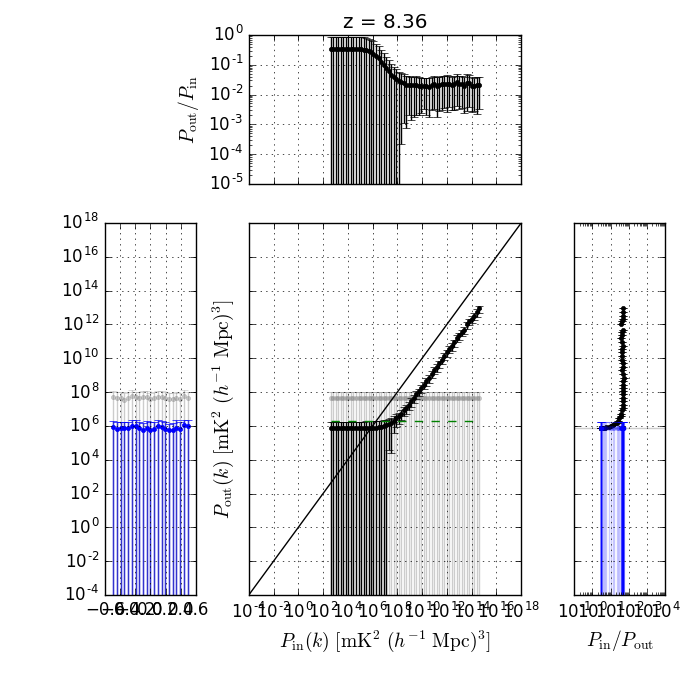
\includegraphics[width=.45\textwidth]{ali_reconstruction_loss_curve.png}
%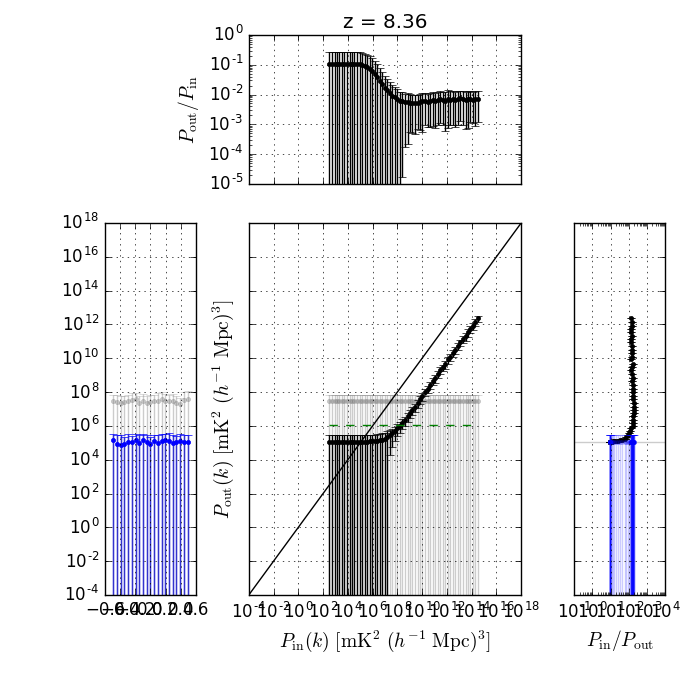
\includegraphics[width=.45\textwidth]{data/optimal_data_loss_curve.png}
\caption{Left: A15 Loss curve. %Right: Optimal FRF loss curve 
{\bf \color{red} these figures are awful but are mostly filling space currently until we make 'em pretty} \label{fig:sigloss_data}}

\end{figure}


\begin{figure}[t]
\centering
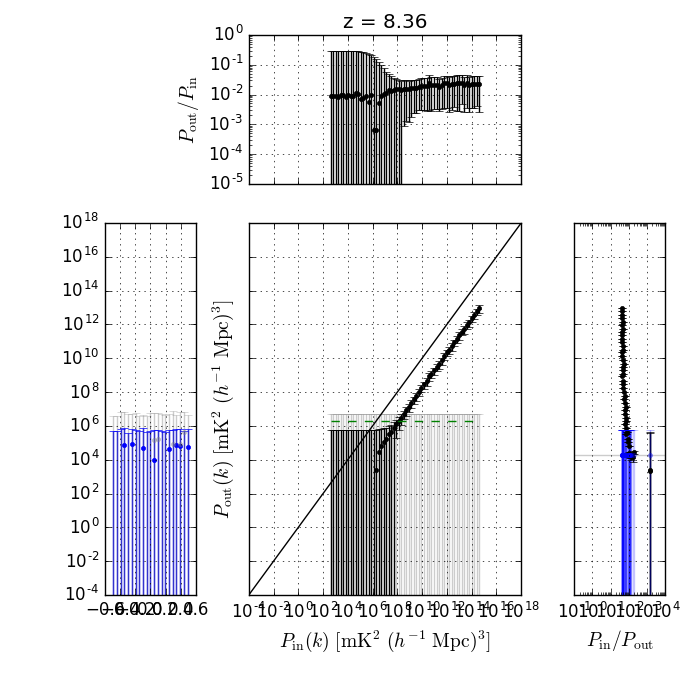
\includegraphics[width=.45\textwidth]{ali_noise_loss_curve.png}
%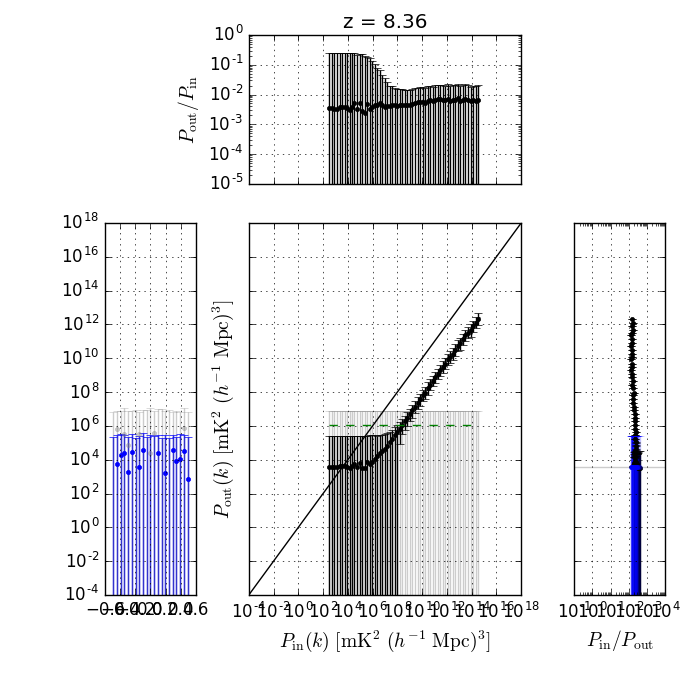
\includegraphics[width=.45\textwidth]{data/optimal_noise_loss_curve.png}
\caption{Left: A15 Loss curve noise. %Right: Optimal FRF loss curve noise 
{\bf \color{red} these figures are awful but are mostly filling space currently until we make 'em pretty} \label{fig:sigloss_noise}}
\end{figure}


\section{Discussion}\label{sec:discussion}{

}

\bibliographystyle{apj}
\bibliography{biblio}


\end{document}